\section{AreaComp V3}

In Version 3 des Algorithmus werden die Wahl der LCP-Intervalle, die in Betracht gezogen werden sollen, eingeschränkt. Ebenfalls werden die in V2 eingeführten Datenstrukturen $\texttt{ruleIntervals}$ und $\texttt{ruleIntervalStarts}$ durch eine effizientere Datenstruktur ersetzt, um effizienteres Markieren von Ersetzungsintervallen zu ermöglichen. 

\subsection{Wahl der LCP-Intervalle}
\label{lcpchoice}

Die Grundlage hierfür bieten die Abouelhoda-Intervalle von Abouelhoda et al. \cite{abouelhoda_optimal_2002}.
Hierzu ist nötig, dass an den Eingabestring $s := s_1s_2\dots s_{n-1}$ noch ein Symbol $\$$ an $s$ angehängt wird, das lexikographisch größer ist als alle $s_i$ mit $i \in [0..n-1]$. Der in diesem Algorithmus verarbeitete String ist also $s\$ = s_1s_2\dots s_{n-1}\$$
\begin{figure}
	\centering
    \begin{tabular}{c|c|c|c|c|c|c|c|c|c|c|c|c|c|c|}
        \multicolumn{1}{c}{$i$} & \multicolumn{1}{c}{$0$} & \multicolumn{1}{c}{$1$} & \multicolumn{1}{c}{$2$} & \multicolumn{1}{c}{$3$} & \multicolumn{1}{c}{$4$} & \multicolumn{1}{c}{$5$} & \multicolumn{1}{c}{$6$} & \multicolumn{1}{c}{$7$} & \multicolumn{1}{c}{$8$} & \multicolumn{1}{c}{$9$} & \multicolumn{1}{c}{$10$} & \multicolumn{1}{c}{$11$}\\\cline{2-13}
        $s$   & a & a & b & a & a & c & a & a & b & a & a & \$\\\cline{2-13}
        $SA$  & 0 & 6 & 3 & 9 & 1 & 7 & 4 & 10 & 2 & 8 & 5 & 11\\\cline{2-13}
        $LCP$ & 0 & 5 & 2 & 2 & 1 & 4 & 1 & 1 & 0 & 3 & 0 & 0\\\cline{2-13}
    \end{tabular}
    \caption{Suffix-Array und LCP-Array für den String $abracadabra\$$, wobei $\$$ das lexikographisch größte Zeichen ist.}
    \label{v3lcparrexample}
\end{figure}

Betrachte \autoref{v3lcparrexample}.
Es gilt nun zu entscheiden, welche Intervalle im zugehörigen \emph{Suffix-Array} einen wiederholt auftretenden Substring bezeichen, dessen Substitution eine möglichst gute Kompression erzielt.
Wir suchen hier Intervalle im Suffix-Array im Gegensatz zu Intervallen im LCP-Array, da die in \cite{abouelhoda_optimal_2002} beschriebenen Algorithmen Intervalle im Suffix-Array erwarten. (siehe \autoref{abouelhodaintervals})
Da aber die relevanten LCP-Werte für ein Intervall im Suffix-Array $SA[i..j]$ mit $i < j$ durch das LCP-Intervall $LCP[i+1..j]$ gegeben sind, ist dies nicht weiter problematisch. 

Betrachten wir das Intervall $SA[0..2]$.
Die zugehörigen LCP-Werte stehen dann in $LCP[1..2]$ und der LCP auf diesem Intervall ist $2$, da $LCP[1] = 5$ und $LCP[2] = 2$. Allerdings kann das Intervall im Suffix-Array auch $SA[0..3]$ gewählt werden, ohne die Länge des längsten gemeinsamen Präfix zu verringern, da auch $LCP[3] \geq 2$ ist. 
Es folgt also, dass es keinen Nutzen hat, das Intervall $SA[0..2]$ gegenüber $SA[0..3]$ zu betrachten, da durch $SA[0..2]$ ein Vorkommen des gleichen Musters missachtet wird.

Wir benötigen also nur die lokal größtmöglichen Intervalle, die für einen bestimmten längsten gemeinsamen Präfix möglich sind. Die Abouelhoda-Intervalle aus \cite{abouelhoda_optimal_2002} dienen diesem Zweck und erlauben es uns, gerade die Intervalle zu wählen, die \emph{sämtliche} Vorkommen eines bestimmten Substrings liefern. Durch das Kind-Array können all diese Intervalle bestimmt werden, indem für jedes Abouelhoda-Intervall die Kind-Intervalle bestimmt werden und dies rekursiv fortgesetzt wird. 

Für unsere Zwecke sind nur $\ell-$Intervalle von Bedeutung, für die $\ell \geq 2$ gilt, da Substrings mit Länge kleiner als zwei keine mögliche Kompression durch Substitution bieten.

Es werden also nun statt allen möglichen Intervallen nur die Abouelhoda-Intervalle berechnet, indem rekursiv die Kind-Intervalle des Wurzel-Intervalls ($[0..n-1]$) berechnet werden. Damit reduziert sich die Anzahl der Intervalle auf $\mathcal{O}(n)$. Denn:

\paragraph{Beweis}
Zu zeigen: Für ein Abouelhoda-Intervall $I$ ist die Gesamtanzahl $m_I$ der Kind-Intervalle, Enkel-Intervalle etc., sich selbst eingeschlossen, durch $|I|$ nach oben beschränkt. Beweis per Induktion über die Länge des Abouelhoda-Intervalls $I$.

\subparagraph{IA: $u = 2$}
Sei $I$ ein Abouelhoda-Intervall mit $|I| = u = 2$. Dann hat $I$ keine Kind-Intervalle und die die Gesamtanzahl der gesuchten Intervalle ist $m_I = 1 \leq u$.

\subparagraph{IV:} Für ein Abouelhoda-Intervall $I$ mit $|I| \leq u$ ist die Anzahl $m_I$ aller Kind-Intervalle, Enkel-Intervalle etc., sich selbst eingeschlossen, durch $u$ beschränkt.

\subparagraph{IS: $u \rightarrow u + 1$}

Sei $I$ ein Abouelhoda-Intervall mit $|I| = u+1$ und $i_1, \dots, i_k \in I$ mit $i_0 < \dots < i_k$ die $\ell$-Indizes von $I$ für ein $\ell \in \mathbb{N}$. Dann sind $I_0 := [0..i_1-1], I_1 := [i_1..i_2-1], \dots I_k := [i_k..u]$ die Kind-Intervalle von $I$. (siehe \autoref{embeddedlcpintervals}) Es gilt dann mit $IV$ für alle $I_j$, dass die Anzahl der gesuchten Intervalle $m_{I_j} \leq |I_j|$ ist.

Für die Anzahl der Intervalle von $I$ gilt dann:
\begin{equation*}
    m_I = 1 + \sum_{i=0}^k m_{I_i} \leq 1 + \sum_{i=0}^k |I_k| = |I| + 1 = u + 1
\end{equation*}
Damit ist die Behauptung gezeigt. $\square$\\\\
Für das LCP Intervall des Eingabestrings ist dann also die Anzahl der Abouelhoda-Intervalle in $\mathcal{O}(n)$. 

\subsection{RuleIntervalIndex}
\label{riiv3}

Ein weiteres Problem sind die Datenstrukturen $\texttt{ruleIntervals}$ und $\texttt{ruleIntervalStarts}$. Diese sind sowohl im Bezug auf Speicher als auch Laufzeit ineffizient. Die Lösung für dieses Problem bietet die Datenstruktur $\texttt{RuleIntervalIndex}$.

Diese basiert auf einer assoziativen Predecessor-Datenstruktur \cite{dinklage_engineering_2021} und unterstützt auch entsprechende Anfragen. Hier wird zu diesem Zweck eine assoziative Variante von Red-Black-Trees \cite{bayer_symmetric_1972, guibas_dichromatic_1978} verwendet (\texttt{TreeMap} in Java). Diese hat eine Laufzeit von $\mathcal{O}(\log n)$ bei allen Operationen der Predecessor-Datenstruktur. 

In der Predecessor-Datenstruktur ordnen wir jeweils immer einen Startindex dem am tiefsten verschachtelten Ersetzungsintervall zu, der an diesem Index beginnt. Dabei kann es vorkommen, dass etwa ein kleineres und tieferes Intervall, in einem größeren Intervall liegt. Deswegen werden die Ersetzungsintervalle nicht ganz, sondern in Teilen gespeichert.

Im Folgenden bezeichnet $R_k$-$[i..j]$ einen Teil eines Ersetzungsintervalls der Regel $k$, der das Intervall $[i..j]$ mit $i \leq j$ belegt. 

Betrachte \autoref{v3ruleintervalindex}. Die Intervallteile $R_1$-$[0..0]$ und $R_1$-$[3..3]$ gehören demselben Ersetzungsintervall $[0..3]$ an. Dies ist insbesondere in der entsprechenden $\texttt{ruleIntervals}$ Datenstruktur in \autoref{v2datastructures} sichtbar. Da allerdings das Ersetzungsintervall $[1..2]$ der Regel $R_2$, und der entsprechende Intervallteil $R_2$-$[1..2]$ tiefer verschachtelt ist, als $[0..3]$, muss an den Indizes $1$ bis $2$ $[1..2]$ gespeichert werden.

Die Elemente der Datenstruktur sind Teile von Ersetzungsintervallen und die Schlüssel die Startindizes der Intervall-Teile. Im Code heißen diese $\texttt{RuleInterval}$. Diese enthalten folgende Attribute:
\begin{itemize}[leftmargin=2.5cm]
	\item[\texttt{ruleId}] Die Regel, die dieses Intervall repräsentiert
	\item[\texttt{start}] Der Start-Index dieses Intervall-Teils
	\item[\texttt{end}] Der End-Index dieses Intervall-Teils
	\item[\texttt{totalStart}] Der Start-Index des gesamten Ersetzungsintervall, dem dieser Teil angehört
\end{itemize}

\begin{figure}
	\centering
	
	\begin{tikzpicture}
		
		\matrix (A) [matrix of nodes, nodes={draw, minimum size=7mm, anchor=center}, column sep=-\pgflinewidth]{
            |[draw=none]| $a$ & |[draw=none]| $bc$ & |[draw=none]| $d$ & |[draw=none]| $bc$ & |[draw=none]| $a$ & |[draw=none]| $bc$ & |[draw=none]| $d$ & |[draw=none]| $e$\\
			$R_1$-$[0..0]$ & $R_2$-$[1..2]$ & $R_1$-$[3..3]$ & $R_2$-$[4..5]$ & $R_1$-$[6..6]$ & $R_2$-$[7..8]$ & $R_1$-$[9..9]$ & $R_0$-$[10..10]$\\
		};
		
	\end{tikzpicture}
    \caption{Die entsprechende \texttt{RuleIntervalIndex} Datenstruktur für die Grammatik aus \autoref{v2datastructures}}
    \label{v3ruleintervalindex}
\end{figure}

So kann der Speicherverbrauch gegenüber $\texttt{ruleIntervals}$ und $\texttt{ruleIntervalStarts}$ verringert werden. 

Seien $k$ Elemente in der Datenstruktur gespeichert.
$\texttt{ruleIntervals}$ benötigte eine Laufzeit von $\mathcal{O}(1)$ um zu bestimmen, welche die tiefste Regel an einem Index $i$ ist. Diese Laufzeit verschlechtert sich bei $\texttt{RuleIntervalIndex}$ auf $\mathcal{O}(\log k)$, wegen des zugrundeliegenden Red-Black-Trees.

Allerdings verbessert sich die Laufzeit, wenn der Startindex eines Ersetzungsintervalls bestimmt werden soll. Mit $\texttt{ruleIntervals}$ und $\texttt{ruleIntervalStarts}$ benötigte dies $\mathcal{O}(n)$ Laufzeit. Mit $\texttt{RuleIntervalIndex}$ ist dies ebenfalls in $\mathcal{O}(\log k)$ möglich, da nur der tiefste Intervall-Teil bestimmt werden muss ($\mathcal{O}(\log k)$) und dann auf das $totalStart$ Attribut werden kann, um den Startindex des Ersetzungsintervalls zu bestimmen.

Zwar ist theoretisch $k \in \mathcal{O}(n)$, allerdings ist die Anzahl von Elementen in der Predecessor-Datenstruktur in der Praxis nicht unbedingt nahezu $n$, da es meistens viel weniger Ersetzungsintervalle gibt, als Zeichen im Text. Daher ist die Laufzeit dieser Operationen in der Regel besser, als $\mathcal{O}(\log n)$.

\subsubsection{Operationen}

$\texttt{RuleIntervalIndex}$ unterstützt die folgenden Operationen:

\begin{itemize}[leftmargin=5cm]
	\item[$\texttt{mark(id, start, end)}$] Fügt ein neues Ersetzungsintervall $[start.. end]$ in die Datenstruktur ein für die Regel-ID $\texttt{id}$. Dies ist die aufwendigste Operation dieser Datenstruktur. 
    Einerseits können die Grenzen $\texttt{start}$ und $\texttt{end}$ innerhalb anderer $\texttt{RuleInterval}$s $R_s$-$[i_s..j_s]$ und $R_e$-$[i_e.. j_e]$ mit jeweils $i_s \leq start \leq j_s$ und $i_e \leq end \leq j_s$ liegen. Diese müssen dann geschrumpft werden, indem $R_s$-$[i_s..j_s]$ durch $R_s$-$[i_s..start - 1]$ und $R_e$-$[i_e..j_e]$ durch $R_e$-$[end + 1..j_e]$ ersetzt wird. Gilt $i_s = start$ oder $j_e = end$, so werden $R_s$-$[i_s..j_s]$ und $R_e$-$[i_e.. j_e]$ stattdessen gelöscht.
    Zusätzlich müssen dann $R_{id}$-$[start..j_s]$ und $R_{id}$-$[i_e..end]$ einfügt werden, als jeweils erster und letzter Intervall-Teil des neuen Ersetzungsintervalls.
    
    Nun muss für die \texttt{RuleInterval}s, die Teilintervalle von $[j_s + 1..i_e - 1]$ sind, entschieden werden, ob das zugehörige gesamte Ersetzungsintervall tiefer verschachtelt ist als $[start.. end]$.
    Ist das \emph{nicht} der Fall für ein $R_a$-$[i_a..j_a] \subset [j_s + 1..i_e - 1]$, so muss $R_a$-$[i_a..j_a]$ durch ein Intervall $R_{id}$-$[i_a..j_a]$ ersetzt werden. Um dies effizienter zu machen, werden aufeinander folgende \texttt{RuleInterval}s, die weniger tief verschachtelt sind als $[start.. end]$, zu einem neuen \texttt{RuleInterval} für $R_{id}$ verschmolzen.

    Falls $R_a$-$[i_a..j_a]$ tiefer verschachtelt ist als $[start.. end]$, so bleibt $R_a$-$[i_a..j_a]$ erhalten. 

    Das ersetzen dieser Intervall-Teile kann durch Iteration der Datenstruktur im Bereich $[j_s + 1..i_e - 1]$ umgesetzt werden. 
	\item[$\texttt{intervalContaining(index)}$] Gibt den Intervall-Teil des am tiefsten verschachtelten Ersetzungsintervalls zurück, in dem $\texttt{index}$ enthalten ist. Dies ist durch einen $\texttt{predecessor(index)}$ Aufruf auf der zugrundeliegenden Predecessor-Struktur möglich.
\end{itemize}
































Mithilfe dieser Operationen ist es nun möglich, effizienter zu bestimmen, welches das am tiefsten verschachtelte Intervall an einem Index ist. Dies ist einerseits für die Vorverarbeitung der Vorkommen eines zu ersetzenden Musters wichtig. Hier muss festgestellt werden, ob ein Vorkommen ersetzt werden darf. Dazu muss unter Anderem geprüft werden, ob die Grenzen des entstehenden Ersetzungsintervalls in demselben bereits bestehenden Ersetzungsintervall liegen. 

Andererseits ist dies auch für das tatsächliche Ersetzen eines Musters wichtig, um festzustellen in welcher Regel das sich das jeweilige Vorkommen befindet und ersetzt werden muss.

\subsection{Kleinere Verbesserungen in der Rule Datenstruktur}

In V2 bestehen die Regeln aus zwei dynamischen Arrays, die einerseits die Symbole selbst (\texttt{symbols}), und andererseits die Präfixsumme über die Länge der einzelnen Symbole speichert (\texttt{cumulativeLength}).
Die Position eines Terminals in der vollständig expandierten Form von \texttt{symbols} wird durch eine binäre Suche auf \texttt{cumulativeLength} berechnet. Die Suche von Symbolen ist zwar effizient, nur ist das Ersetzen von Bereichen in diesen Arrays ineffizient. Denn hier, muss ein Bereich aus diesen Arrays gelöscht, und durch ein Nichtterminal ersetzt werden. Dies hat eine Laufzeit von $\mathcal{O}(n)$ für eine Regel mit $n$ Symbolen.

In V3 wurden diese durch einen assoziativen Red-Black-Tree ersetzt, wie auch in \texttt{RuleIntervalIndex}. Hier wird der Startindex des Symbols in der vollständig expandierten Form dieser Regel als Schlüssel verwendet. Der assoziierte Wert ist dann das Symbol selbst. Betrachten wir beispielsweise diese Arrays aus V2:

\begin{figure}[H]
	\centering
	\subfloat[symbols]{
		\begin{tabular}{|c|c|c|c|c|c|} \hline
			$R_1$ & $a$ & $b$ & $R_3$ & $R_2$ & $d$ \\\hline
		\end{tabular}
	}
	\quad
	\subfloat[cumulativeLength]{
		\begin{tabular}{|c|c|c|c|c|c|} \hline
			$5$ & $6$ & $7$ & $12$ & $18$ & $19$ \\\hline
		\end{tabular}
	}
\end{figure}

In V3 würden diese stattdessen etwa folgendermaßen dargestellt werden:

\begin{figure}[H]
	\centering
	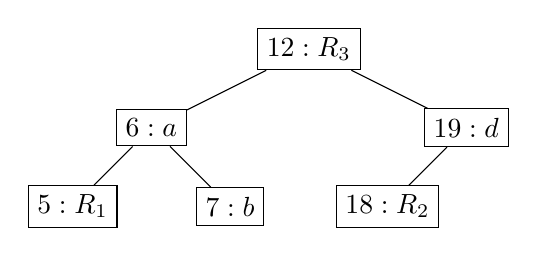
\begin{tikzpicture}
		
		\node[draw] (12) at (0,0) {$12: R_3$};
		\node[draw] (6) at (-2, -1) {$6: a$};
		\node[draw] (19) at (2, -1) {$19: d$};
		\node[draw] (18) at (1, -2) {$18: R_2$}; 
		\node[draw] (5) at (-3, -2) {$5: R_1$};
		\node[draw] (7) at (-1, -2) {$7: b$};
		
		\draw[-] (12) -- (6);
		\draw[-] (6) -- (5);
		\draw[-] (6) -- (7);
		\draw[-] (12) -- (19);
		\draw[-] (19) -- (18);
		
	\end{tikzpicture}
\end{figure}

Sei also ein Baum mit $n$ Elementen gegeben, so wie ein Intervall $[i..j]$, $i <= j$. Liegen nun $k$ Elemente, im Intervall $[i..j]$, so können alle diese Elemente insgesamt in $\mathcal{O}(k \log n)$ Laufzeit entfernt werden, da immer $\mathcal{O}(\log n)$ Laufzeit benötigt wird, um ein Element zu finden.

\subsection{Probleme}
\label{v3problems}

Die Laufzeit ist durch die beschränkte Wahl der LCP-Intervalle, \texttt{RuleIntervalIndex} und die Verbesserte Regel-Datenstruktur, erheblich verbessert, aber es gibt trotzdem noch Probleme mit V3.

\subsubsection{Speicherverbrauch}
Da V3 als erste Version auch auf Datenmengen größer als 1MB tolerable Laufzeiten erzielt, stellt sich als nächstes das Problem des Speicherverbrauchs. Allein auf einer Datenmenge von 50MB, benötigte V3 schon etwa 6-8GB oder mehr.

\subsubsection{Effizienz von RuleInvervalIndex}

Außerdem ist \texttt{RuleIntervalIndex} nicht optimal. Viele der Operationen benötigen noch mehrere Anfragen an die darunterligende Predecessor-Datenstruktur.\\
Um etwa für einen Index $i$ den Intervall-Teil des Ersetzungsintervalls zu erhalten in dem $\texttt{i}$ liegt, muss zuerst ein $\texttt{predecessor(i)}$ Aufruf durchgeführt werden, um den Intervall-Teil $\texttt{part}$zu erhalten in dem $\texttt{i}$ liegt. Dann muss eine $\texttt{get(part.totalStart)}$ Anfrage durchgeführt werden, um den ersten Intervall-Teil zu erhalten.\\
Diese Anfrage kommt oft vor, da sie benötigt wird, um zu entscheiden, ob ein Vorkommen eines Musters ersetzt werden darf.

Dazu ist das markieren, also das einfügen neuer Ersetzungsintervalle noch kostspielig. Dies benötigt ebenfalls mehrere Anfragen an die Predecessor-Struktur. Außerdem müssen für das neu einzufügende Intervall $[start, end]$ alle Intervalle mit Startpositionen im Bereich $[start, end]$ durchlaufen werden, um diese potentiell zu ersetzen, falls diese weniger tief verschachtelt sind, als das neu einzufügende Intervall. Dies kann im Worst-Case lineare Laufzeit in der Länge der Eingabe bedeuten.

\subsubsection{Zu strenge Entscheidung ob Vorkommen ersetzt werden dürfen}
\label{strictdecision}
Ein weiteres Problem ist bei der Entwicklung dieser Datenstrukturen aufgefallen. Es gibt fälle, in denen die bisher geschriebenen Algorithmen eine Ersetzung verbieten, obwohl diese eigentlich legal wäre.

Sei $p$ ein Muster mit Länge $k := |p|$. Bisher wird entschieden, ob eine Substitution von $p$ bei Index $i$ legal ist, indem geprüft wird, ob $\texttt{intervalContaining(i)}$ und $\texttt{intervalContaining(i + k - 1)}$ dieselben $\texttt{ruleId}$ und $\texttt{totalStart}$ besitzen, also die Start- und Endposition des neu entstehenden Ersetzungsintervalls in demselben Ersetzungsintervall liegen. Falls dies der Fall ist, ist eine Ersetzungs auch tatsächlich immer legal. Allerdings übersieht diese Berechung einen Fall:

Betrachten wir beispielsweise die folgende Grammatik für den String $abcdeabcd$:
\begin{align*}
	R_0 &\rightarrow R_1 c d e R_1 c d\\
	R_1 &\rightarrow a b\\
\end{align*}
Angenommen, als nächstes soll das Muster $abcd$ ersetzt werden (beachte, die Muster sind immer bezüglich des Eingabestrings, da das Suffix- und LCP array für diesen berechnet sind).
\texttt{RuleIntervalIndex} sieht hier folgendermaßen aus:
\begin{figure}[H]
	\centering
	\begin{tabular}{|c|c|c|c|} \hline
		$R_1$-$[0..1]$ & $R_0$-$[2..4]$ & $R_1$-$[5..6]$ & $R_0$-$[7..8]$ \\\hline
	\end{tabular}
\end{figure}

Das Muster $abcd$ kommt bei den Indizes $[0, 5]$ vor. Beide Ersetzungen sind offensichtlich legal, indem eine neue Regel $R_2 \rightarrow R_1cd$ eingeführt wird.\\ Versucht man aber nun mit der bisherigen Methode zu prüfen, ob die Ersetzung legal ist, so, erhält man:
\begin{align*}
	I_1 &:= \texttt{intervalContaining(0)} = R_1\text{-}[0..1]\\
	I_2 &:= \texttt{intervalContaining(0 + 4 - 1)} = R_0\text{-}[2..4]
\end{align*} 
Dabei ist dann $1 = I_1.ruleId \neq I_2.ruleId = 0$ und $0 = I_1.totalStart \neq I_2.totalStart = 2$. Die Ersetzung wird also verweigert, obwohl diese eigentlich legal wäre.\\
Diese Fälle treten ein, wenn das erste oder letzte Zeichen des zu ersetzenden Musters ein Nichtterminal ist (das Muster $abcd$ lag in der Grammatik bereits als das ersetzte $R_1 cd$ vor).

\texttt{RuleIntervalIndex} bietet zu diesem Zeitpunkt nicht die Daten um diesen Fall effizient korrekt zu entscheiden.